%=========================
% Materials and Methods
%=========================
%============NOTE==============
% Check tense !!! It should be past tense and mostly passive voice.
%==============================
This research mainly examined relationships between the injuries caused by pests and diseases, cropping practices (e.g., rice variety grown, crop establishment method, fertilizer and chemicals applied), and rice yields using data collected from surveys of irrigated lowland rice growing areas in South and South East Asia. Their relationships were constructed and analyzed by network analysis. I developed and applied suitable methods of network analysis to characterize the associations of injuries and cropping practices. The resulting network of associations of injuries and cropping practices thus provided a starting point for further investigations of their relationships (i.e., comparison of networks under different production environments or examination of networks at different levels of yield gains). 
% You're still changing tense. Once I tell you to fix something, please fix it. Do not repeat the mistake. 
% Grammar in last sentence

Network analysis of rice crop health survey data was divided into three parts. In the following, I presented three distinct network analysis approaches: single-network analysis, differential network analysis, and dynamic network analysis. Three approaches answered different questions. I applied single-network analysis to the data from all fields surveyed for identifying patterns of interactions  between injuries and cropping practices and key components (e.g., most connected variables). Second, differential network analysis aimed to uncover similarities and differences of networks constructed from the different data sets (e.g., dry season versus wet season). Dynamic network analysis was applied to study on how networks changed under at least two different aspects of an evolving complex system. Here, I focused on the dynamic networks under different levels of yield gains. 

\subsection*{Crop Health Survey Data}
\addcontentsline{toc}{chapter}{Crop health survey data}

%Rice is dominantly produced in Asia, 31 percent of the global rice harvested comes from Southeast Asia \shortcite{oecd2012oecd}. The highest levels of productivity are found in irrigated areas, where is the most intensified production system. Farmers can grow rice more than one crop per year here. Approximately 45 percent of the rice growing area in Southeast Asia is irrigated, with the largest areas being found in Indonesia, Viet Nam. Philippines and Thailand \shortcite{mutert2002developments}. In South Asia, major rice-growing countries are India and Bangladesh. India has the largest rice growing area (approximately 43 million hectares) in the world and contributes 25 percent of global rice production. 

The crop health survey data were collected through surveys of farmers' fields in two seasons (wet and dry seasons) from 2009 to 2015 in different production environments across South and South East Asia in irrigated lowland rice growing areas (West Java, Indonesia; Mekong River Delta and Red River Delta, Vietnam; Tamil Nadu and Odisha, India; and Suphanburi, Thailand). The survey protocol based on the "Survey Portfolio" described by \shortciteA{Savarysurvey2009} was used. % is this correct? Was it the 1996 version or the updated version from 2009 that was used? sith:[clear]

%======= Note ================
% don't leave spaces between letters and punctuation marks, e.g., no space after "(" or before "."
% If you're going to use them, learn the difference between i.e. and e.g. they are not the same
%======================================

% Verb tense, here, still
% See note above for both comments. These still are not fixed here!
% You'd best re-read the protocol to familiarise yourself with just what data is collected and correct what you've written here.

The survey data described above consisted of measures of multiple variables. Theses variables were able to classify to three groups: cropping practices, injuries, and actual yield estimates. They are summarized in Table 1. \textbf{cropping practices} included types of rice varieties, crop establishments, amount of fertilizers used, frequency of pesticides application. %\textbf{cropping practice set} was simplified, which collected with many type of data. For example, types of rice varieties (traditional varieties, modern varieties, and hybrid rice), crop establishments ( direct seeded, transplanted rice) were collected in categorical data, pesticide (molluscicide, herbicide, insecticide and fungicide) uses were collected discretized data, and accumulated organic, chemical fertilizers were collected in continuous data. \textbf{Injuries and diseases set} composed of specific signs caused by pests or pathogens (i.e., whitehead, brown spot). They were collected percent of incidence of injury at two rice stages (active tillering and active ripening stage). Two types of injury indices were used areas under progress curves or maximum level of injuries or disease incidence depending on the nature of the injury.
 %The data that were collected at the individual field level were summarized in Table 1. These data were collected during four visits in each field during the rice growing season and described quantitative information on crop growth and levels of injuries to the crop due to pest (pathogens, insects and weeds) over time, as well as yield. Each field surveyed in each year was considered to be unique and was represented by a characteristic set of attributes pertaining to injuries and yield. 
%Injury variables were derived from time-dependent information on diseases, insects and weeds observed at four development stages of the growing crop: tillering, booting, early dough and maturity in such a way that they would best account for possible yield reductions (Savary et al., 1994). While injuries due to diseases and insects were specific to species (or species groups), information on weed infestation was the area covered by any weed species, either above or below the crop canopy.
%Except for weeds, information pertaining to injuries was collected in the form of number of injured organs (tillers, leaves and panicles), which later was made relative to the corresponding total number of organs present in the sampling units (10 hills per field for transplanted rice crops). As for weed infestation, the proportion of soil area covered at two levels of the crop canopy (below or above it) was assessed in three spots of 1 m2 each. Although a very large number of pathogens, insects and weeds are harmful to rice, many are seldom considered to cause yield losses (Teng, 1990b; Willocquet et al., 2004). The study therefore concentrated on injuries listed in Table 1. Data compaction over time during crop growth was necessary to achieve the objective of analysis. 

%For this purpose, two types of injury indices were used: areas under injury progress curves or maximum level at any of the four observations, depending on the nature of the injury (Table 1; Savary et al., 1994, 1996). The area under injury progress curve (AUIPC) (Campbell and Madden, 1990) was calculated by the mid- point method using the following equation:
%$ AUDIP = \sum \frac{1}{(x_{i} + X_{i-1})(T_{i} - T_{i-1})}$
%\begin{tubular}
%\hline
%Variable type & Variable & Variable description & unit \\
%\hline
%\end{tubular}

\section*{Single network analysis of crop health survey data}
\addcontentsline{toc}{chapter}{Single network analysis of crop health survey data}
\textbf{Introduction}

%========================
% use textit{p}-values
%=======================
Cropping practices and injuries profiles network model based on the survey data. It was defined the correlation based network as undirected, weighted network. The nodes of the network corresponded to variables, and edges between variables were determined by the pairwise correlation.

%While this network was focused, it did not imply that only a single data set is used. Instead, appropriately similar multiple data sets can be used to validate the robustness of module definition and connectivity.
% objective
% 1. The rules is to, incorrect grammar
% 2. Capitalization
% 3. Punctuation
A network model based on crop health survey data has not yet been report. Additionally, correlation analysis, and network analysis of these data has not been studied. Thus, evaluation of such methods is challenging. According to \shortciteA{kolaczyk2014statistical}, correlation based network construction has at least three important issues to be encountered. First, there is the choice of pairwise correlation measure to be used. Second, statistic significant must be determined for removal of spares relationships. And third, the problem of multiple testing must be considered because there are large number of tests of pairwise comparison.

%An overview of cropping practices and injuries profiles network construction was depicted in Fig. 1: (a) data processing, (b) calculate correlation coefficients (Pearson, Spearman, or Kendall). Estimate \textit{p}-values for all coefficients. Next, determine threshold values for the resulting correlation coefficients will stored in adjacency matrices for the construction of networks, (c) Construct a network model, analyze network properties.

%The use of crop health survey data to construct co-occurrence network and perform network decomposition and network analysis has not yet been reported. Additionally, methods performing co-occurrence analysis and co-occurrence networks has not been studied. Thus, evaluation of such methods is challenging because there are many types of variables mixed in crop health survey data; methods can identify variables with true concordance often determine the prior knowledge; and methods performing biologically meaningful co-occurrence network construction. 

% The following comment is still not corrected.
% the rules is to present is not grammaticaly correct

%By raising the absolute value of the Pearson correlation to a power 1 (soft thresholding), the weighted gene coexpression network construction emphasizes large correlations at the expense of low correlations. Specifically, 
% methods

\textit{\textbf{Network construction}}

% Again, I'm still confused, is this written in past tense (like a normal paper) current (which doesn't make sense) or future (like a proposal should be)? Your verb tenses are not consistent
%========================note====================================
% I typically refer to R functions as "function()" to indicate that it is a function, not just a name or a package, e.g. corr.test(), bicor(), etc. You have no standard in your paragraph to identify R functions, that I can see, you use several ways.
%==========================================================================
% Your last sentence is confusing and incomplete at best, nonsense at worst.

% This whole paragraph needs to be cleaned up, see my comments from previous.

%%% I'm stopping here. You need to spend some time cleaning this section up and making corrections.
Edges of cropping practice and injury profiles network express the degree of correlation between two variables. A standard measurement of correlation between two variable $x$ and $y$ represent $cor(x,y)$, where has values between -1 to +1 depending on the level of relationships. $cor(x_{i}, x_{j})$ equal -1 when there is a decreasing relationship between $x$ and $y$, and +1 when there is a increasing relationship.

To identify the most suitable pairwise correlation methods, I will evaluate four correlation based measures, Pearson's correlation, Spearman's rank correlation, Kendall's correlation, and biweight midcorrealtion. R was employed to compute pairwise correlation \shortcite{R:2014a}. The "\texttt{cor.test()}" function was applied for generating a correlation matrix, which describes the pairwise correlations between variables. This function allows users to choose types of correlation measures to perform such as Pearson's correlation, Spearman's rank correlation and Kandell's rank correlation. To compute biweight midcorrelation, I applied "\texttt{bicor()}" function of WGCNA package \shortcite{Langfelder:2008bd} in R. 

When a correlation matrix was create, next is to construct the correlation based network from the resulting correlation matrix. However, \textit{p}-values should be concerned. As issues mentioned above, \textit{p}-values must be adjusted for multiple testing. Benjamini-Hochberg adjustment or Bonferonni correction are recommended by \shortciteA{kolaczyk2014statistical}, which R function "\texttt{p.adjust()}" can calculate adjusted \textit{p}-values. Alternatively, they are adjusted through control of the false discovery rate. The R package \textbf{fdrtool} can be implemented for this method \shortcite{fdrtool}.

Up until this point, a network model can be created from a correlation matrix, and assessed basic properties. R packages for network analysis, \textbf{igraph} \ shortcite{Csardi:2010wx}, \textbf{qgraph} \shortcite{qgraph}, \textbf{statnet}, \textbf{network} \shortcite{networkpackage}, \textbf{sna} containing several functions will be applied for  computing  network algorithms, and decorating network graphs.

A network model may not lead to reveal biological knowledge, even though it was created from a method based on its principle of statistical operation. Resulting network models based on different correlation measures will be evaluated. The most suitable correlation measure is assumed that it will contribute the network that is able to reveal the associations between variables close to the good understandings of biological relationships that crop health survey observed.  
%====================== Comments===================
% why knowledge of biological literature? Why not a good understanding of the biological system that you are monitoring? I think that's more essential and useful
% models cannot reveal knowledge, look up the definition of knowledge. It does not apply here. What do you really mean because it can not be knowledge?
% first sentence, all of them what?
% based on what study? Our study? Who is "we"? This is YOUR research. If anything it should be "based on my study" but I'm not clear as to what study you refer to here. Who are the "we" that are suggesting? You're the only author on this manuscript. It's your disseration. There is no, our, us or we. It's only my, me, I here.
% Is "codes" the proper form to use?
%====================================================
\section*{Differential network analysis of crop heath survey data under different seasons and production environments}
\addcontentsline{toc}{chapter}{Differential network analysis of crop health survey data under different season and production environment}

% introduction
Networks can response differently under various environments or with external signals.They can be more simplify by focusing on key components and capturing only the essential components differently responding between environments which they play a key role in the modeled response \shortcite{Peer:2011jd}. Networks are examined by adding or depleting some variables. This allows predicting interactions or components that change following the changed structure of networks. 

Differential networks can be used to describe differences between two networks under different conditions. They might display different interactions from the original network. The strongest differential interactions are not necessarily that are strong in static conditions. Conversely, interactions of network under static condition are weak or removed from the differential network. You may infer that if networks constructed from different environment conditions, differential interactions between two networks imply changes that are a result of response to environmental conditions. 

% objective
The objective of differential network analysis is to extract interactions from the original network that appear to be active under different conditions. I focused two aspects of this analysis. The first was to compare how patterns of interactions of cropping practices and injury profile network changed across multiple production environments. The second is to study how networks changed under different seasons. Each data sets was then used to construct the network. Next, these networks were contrasted to find (a) non-preserved modules, (b) differentially occurred variables, and (c) differentially connected variables.
% methods

Based on the methods of single network construction mentioned above, differential networks were constructed from the survey data with different groups of samples following the purpose of network construction. To analyze differential networks under different seasons, I constructed two networks; one was constructed from dry season data, and another was constructed from wet season data. For differential networks of different production environment, they were generated by data set in different locations.

For comparison with a standard differential network analysis, I applied \textbf{WGCNA} \shortcite{horvath2011weighted} and \textbf{dna} \shortcite{dnapackage} package in R, which this package provide several function to analyze the differences of topologies of two networks \shortcite{horvath2011weighted}. 
These packages includes preprocessing tools for simultaneously preparing a pair of networks for analysis, procedures for computing connectivity scores between pairs of variables based on many available statistical techniques, and tools for handling modules of variables based on these scores. Also, procedures are provided for performing permutation tests based on these scores to determine if the connectivity of a variables differs between the two networks, to determine if the connectivity of a particular set of important variables differs between the two networks, and to determine if the overall module structure differs between the two networks. Several built-in options are available for the types of scores and distances used in the testing procedures, and additionally, the procedures provide flexible methods that allow the user to define custom scores and distances.

For example, "\texttt{test.modular.structure()}" function is used to compare between the connectivity measures of each network \shortcite{dnapackage}. 

%I propose the overview of differential networks are illustrated in Figure \ref{fig:wholenet}.


% why is 2.3 not 2.1? % The problem there is that you must put the label after a caption, so the label can reference to the figure (it references to the caption, actually). See here: http://www.latex-community.org/forum/viewtopic.php?t=3659 I've corrected this. - ahs
 

\section*{Dynamic network analysis of crop health survey data}
\addcontentsline{toc}{chapter}{Dynamic network analysis of crop health survey data} % okay edit one more round for more consistancy
% introduction
Networks can dynamically respond and adapt to the internal state and external signals \shortcite{Peer:2011jd}. As the internal state, backgrounds of nodes influence the structure and behavior of the network and give rise to significant differences across individuals. Backgrounds are included information about where the data are from. The different sources and different times collecting the data strongly determine the network behaviors. 

Biological systems are highly dynamic that must continuously respond to a external signals or internal state of the system, or they can be altered more slowly over time \shortcite{Peer:2011jd}. Thus realistically the corresponding network graphs evolve as well, and should be analyzed. It seems clear that if we are able to develop a complete understanding of biological systems, we must understand the systems on how their dynamic effects are, they are affected by, changes in the different conditions. Some understandings were obtained from studies of dynamics of large networks, for example, gene expression or metabolic fluxes network \shortcite{Idekerdiffnet}.

Dynamic network analysis is applied for study changes of networks at least two different aspects of an evolving complex system. The main goal of this analyais move away from characterizing absolute properties of the system to concentrate on a specific dynamic systems response. Rather than answer what the key factors in the system, they answer what parts of the system are most affect by perturbation.

Form the previous study of \shortciteA{Savary:2000vr}, levels of actual yields are affected by different patterns of interactions between injuries and cropping practices. The results from damages of pests and disease will be able to lead to yield loss. Hypothetically, Different yield gains are the consequence of different patterns of interaction between injuries and disease, and production situations.  From the context of crop health survey data, 

My objectives are to construct networks of crop health survey data at different level of farmers' yields. When networks were generate, I will perform dynamic network analysis following \shortcite{kolaczyk2014statistical}. This analysis will enable us to find out how network changed when yield gains decreased or increased.

To obtain the data for constructing the dynamic network, I varied yield gains, and obtain different yield data set in order to construct a dynamic network of yield varying behaviors. I employed \textbf{networkDynamic} \shortcite{networkdynamicpackage} and \textbf{ndtv} \shortcite{ndtvpackage} packages to generate yield-varying networks. The dynamic graphs will be characterized following \shortcite{bilgin2006dynamic, kolaczyk2014statistical}

\subsection*{Analyzing the Structure of Network Models}

% edited for Tex code
Once networks are constructed, several indices can be computed to convey information about network structure. Structural properties of networks can be used for the interpretation of datasets. Two types of structure are important. First, typically one is interested in the global structure of the network (random networks, small networks, scale-free networks) \shortcite{Strogatz:2001wc, Jeger:2007tn}. Second, one may be interested in local patterns, which are characteristics of each node. For example, clustering of nodes and/or edges in a network can identify groups of nodes with similar properties, and these are referred to "modules" or "communities" \shortcite{osorio2012integrative, Jeger:2007tn}.

% edited for clarity
Comparing the networks by using some key topological properties of network is usefully conducted. Node degree and degree distribution are simple properties, which are the number of connections of each node and the frequency distribution of the number of connections per node, respectively. Cluster coefficient is the other measure, which is the value indicating whether or not the entities in network form cluster or group within network structure. \shortciteA{Deng:2012do, Toubiana:2013cv, horvath2011weighted, newman2003structure} are recommended references for descriptions of the network properties as well as the formal calculation of these measures.


%\begin{landscape}

%\begin{figure}[h!]
%\centering
%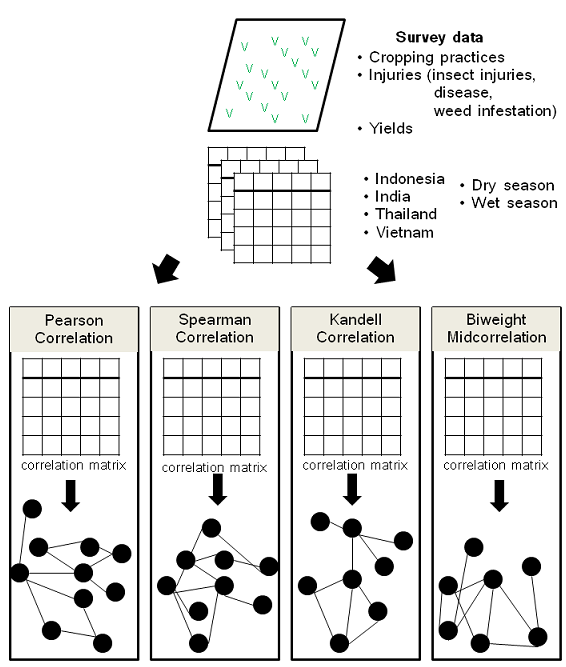
\includegraphics[resolution = 600]{pipeline}
%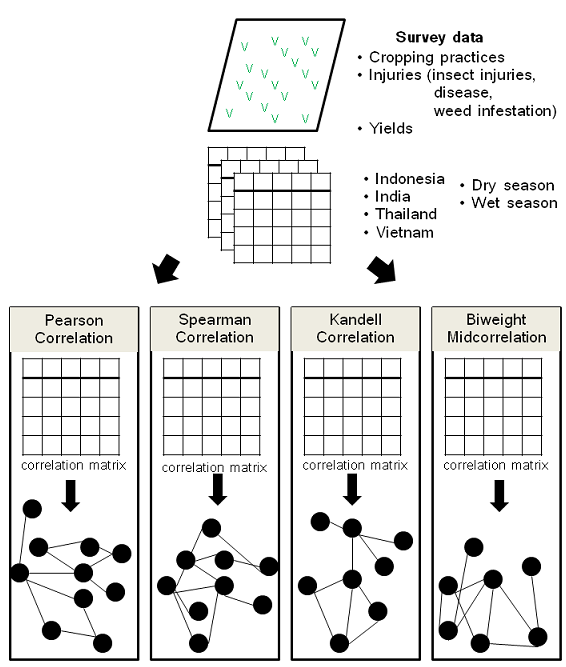
\includegraphics[width=6in]{pipeline}

%\caption[Proposed pipeline for network construction]{Proposed pipeline for network construction. (a) Collect the input profiling data and output profiling data from different samples and different locations. (b) Calculate correlation coefficients (Pearson, Spearman, or Kendall). Estimate P-values for all coefficients. Next, determine threshold values for the resulting correlation coefficients and \textit{P} values, storing results in adjacency matrices for the construction of networks. (c) Construct network and analyze network for graph-theoretic properties and infer biological meanings and integrate the network of input data and output data. (d) Repeat analysis for a second season to verify the network model.}
%\label{fig:pipeline}
%\end{figure}
%\end{landscape}

%\newpage
%\begin{landscape}
%\begin{figure}[h!]
%\centering
%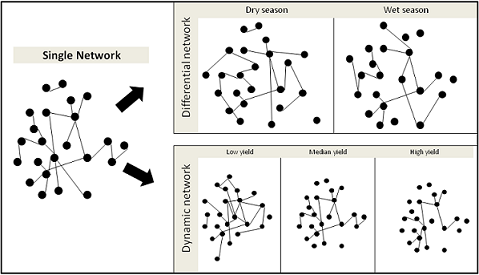
\includegraphics[width=6in]{wholenet}

%\caption[Network comparison]{Network comparison: Network models constructed from survey datasets of different geographic locations are compared by determining their properties. Networks will express the conserved domains within their structure. A merged representation of the two networks being compared is also proposed as a holistic network of rice ecosystem in South and South East Asia.}
%\label{fig:wholenet}
%\end{figure}
%\end{landscape}

%================eos================================

